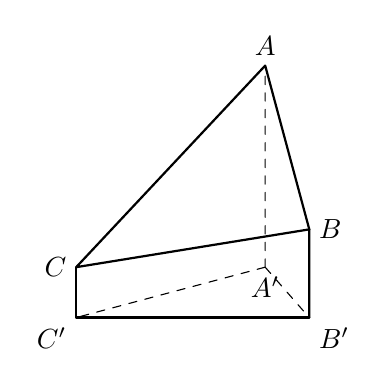
\begin{tikzpicture}[line cap=round,line join=round,scale=0.8]
\usetikzlibrary{calc}

% --- ground plane A'B'C' as a parallelogram ---
\coordinate (Cp) at (0,0);
\coordinate (Bp) at (3.7,0);
\coordinate (Ap) at (3.0,0.8);

\draw[thick]   (Bp) -- (Cp) -- cycle;

% labels on plane
\node[below left]  at (Cp) {$C'$};
\node[below right] at (Bp) {$B'$};
\node[below]       at (Ap) {$A'$};

% --- verticals up to A,B,C ---
\def\hA{3.2}
\def\hB{1.4}
\def\hC{0.8}

\coordinate (A) at ($(Ap)+(0,\hA)$);
\coordinate (B) at ($(Bp)+(0,\hB)$);
\coordinate (C) at ($(Cp)+(0,\hC)$);

\draw[dashed] (Ap) -- (A);
\draw[thick] (Bp) -- (B);
\draw[thick] (Cp) -- (C);

% --- triangle ABC in space ---
\draw[thick] (A) -- (B) -- (C) -- cycle;

% --- some auxiliary dashed lines on the plane (to mimic the sketch) ---
\draw[dashed] (Ap) -- (Bp);
\draw[dashed] (Ap) -- (Cp);

% labels of A,B,C
\node[above] at (A) {$A$};
\node[right] at (B) {$B$};
\node[left]  at (C) {$C$};
\end{tikzpicture}